\section[Legislativa jaderné bezpečnosti]{Postavení provozovatele, státního dozoru a IAEA v jaderné bezpečnosti, legislativní rámec jaderné bezpečnosti}

\subsection{Životní cyklus jaderných zařízení}

\textbf{1) Záměr postavit jaderné zařízení}

\begin{itemize}
    \item Důležité zvážit proč stavět jaderné zařízení, k čemu bude sloužit.
    \item Výstavba a provoz jaderného zařízení je závazek na desítky let.
    \item Velmi důležité pro země, které začínají s jadernou energetikou.
\end{itemize}

\textbf{2) Umístění, hodnocení lokality}

\begin{itemize}
    \item Výběr a zkoumání mnoha lokalit.
    \item Mnoho kritérií, které musí být posouzeny -- zásoby vody, množství spodní vody, seismická činnost, ...
    \item Z mnoha lokalit se vybere nejvhodnější kandidát a následuje velmi detailní vyhodnocení lokality.
\end{itemize}

\textbf{3) Design a licencování}

\begin{itemize}
    \item Kombinuje výsledky vývoje vybraného projektu a požadavků pro danou lokalitu.
    \item Výpočetní ověření projektu.
    \item Specifikace reaktoru a jeho částí.
    \item Projekt může mít mezinárodní licenci a pak je dále schvalován státním dozorem.
    \item Pokud není mezinárodní licence je potřeba projekt licencovat jako součást povolení pro výstavbu.
\end{itemize}

\textbf{4) Výstavba}

\begin{itemize}
    \item Stavební práce.
    \item Výroba jednotlivých komponent reaktoru.
    \item Instalace jednotlivých komponent a zařízení.
    \item Kontroly a testy při výstavbě.
\end{itemize}

\textbf{5) Uvádění do provozu}

\begin{itemize}
    \item Zprovoznění všech systému.
    \item Ověření, že pracují v souladu s projektem.
    \item Kontrola splnění všech kritérií.
\end{itemize}
    
\textbf{6) Provoz}

\begin{itemize}
    \item Provoz reaktoru zahrnuje všechny činnosti, pro které je zařízení určeno.
    \item Provoz na výkonu, údržba, výměna paliva, spouštění reaktoru, ...
\end{itemize}

\textbf{7) Vyřazování z provozu}

\begin{itemize}
    \item Všechny činnosti, které vedou k zrušení kontroly státního dozoru nad jaderným zařízením.
    \item Dvě fáze: dekontaminace a rozebrání.
    \item Vyvezení paliva z reaktoru, odvezení vyhořelého paliva do skladů VJP, rozebrání IO, IIO a IIIO, zrušení pomocných provozů, zboření budov, ...
    \item Postupuje se od neaktivních provozů a budov k aktivním, IO je poslední
\end{itemize}

\textbf{8) Zrušení dozoru nad jaderným zařízením}

Po odstranění všech radioaktivních materiálů a kontaminovaných komponent není dále důvod pro pravidelné kontroly ze strany státního dozoru.

\subsection{Klíčoví hráči při provozu reaktorů}

Při provozu jaderné elektrárny, resp. jaderného reaktoru do toho mohou mluvit a mají s tím co dočinění celkově tři klíčový hráči:

\begin{itemize}
    \item Stát (vláda)
    \item Státní dozor
    \item Provozovatel (držitel licence)
\end{itemize}

Dále bychom neměli opomenout IAEA, možná i NEA a Euratom.

\begin{figure}[H]
    \centering
    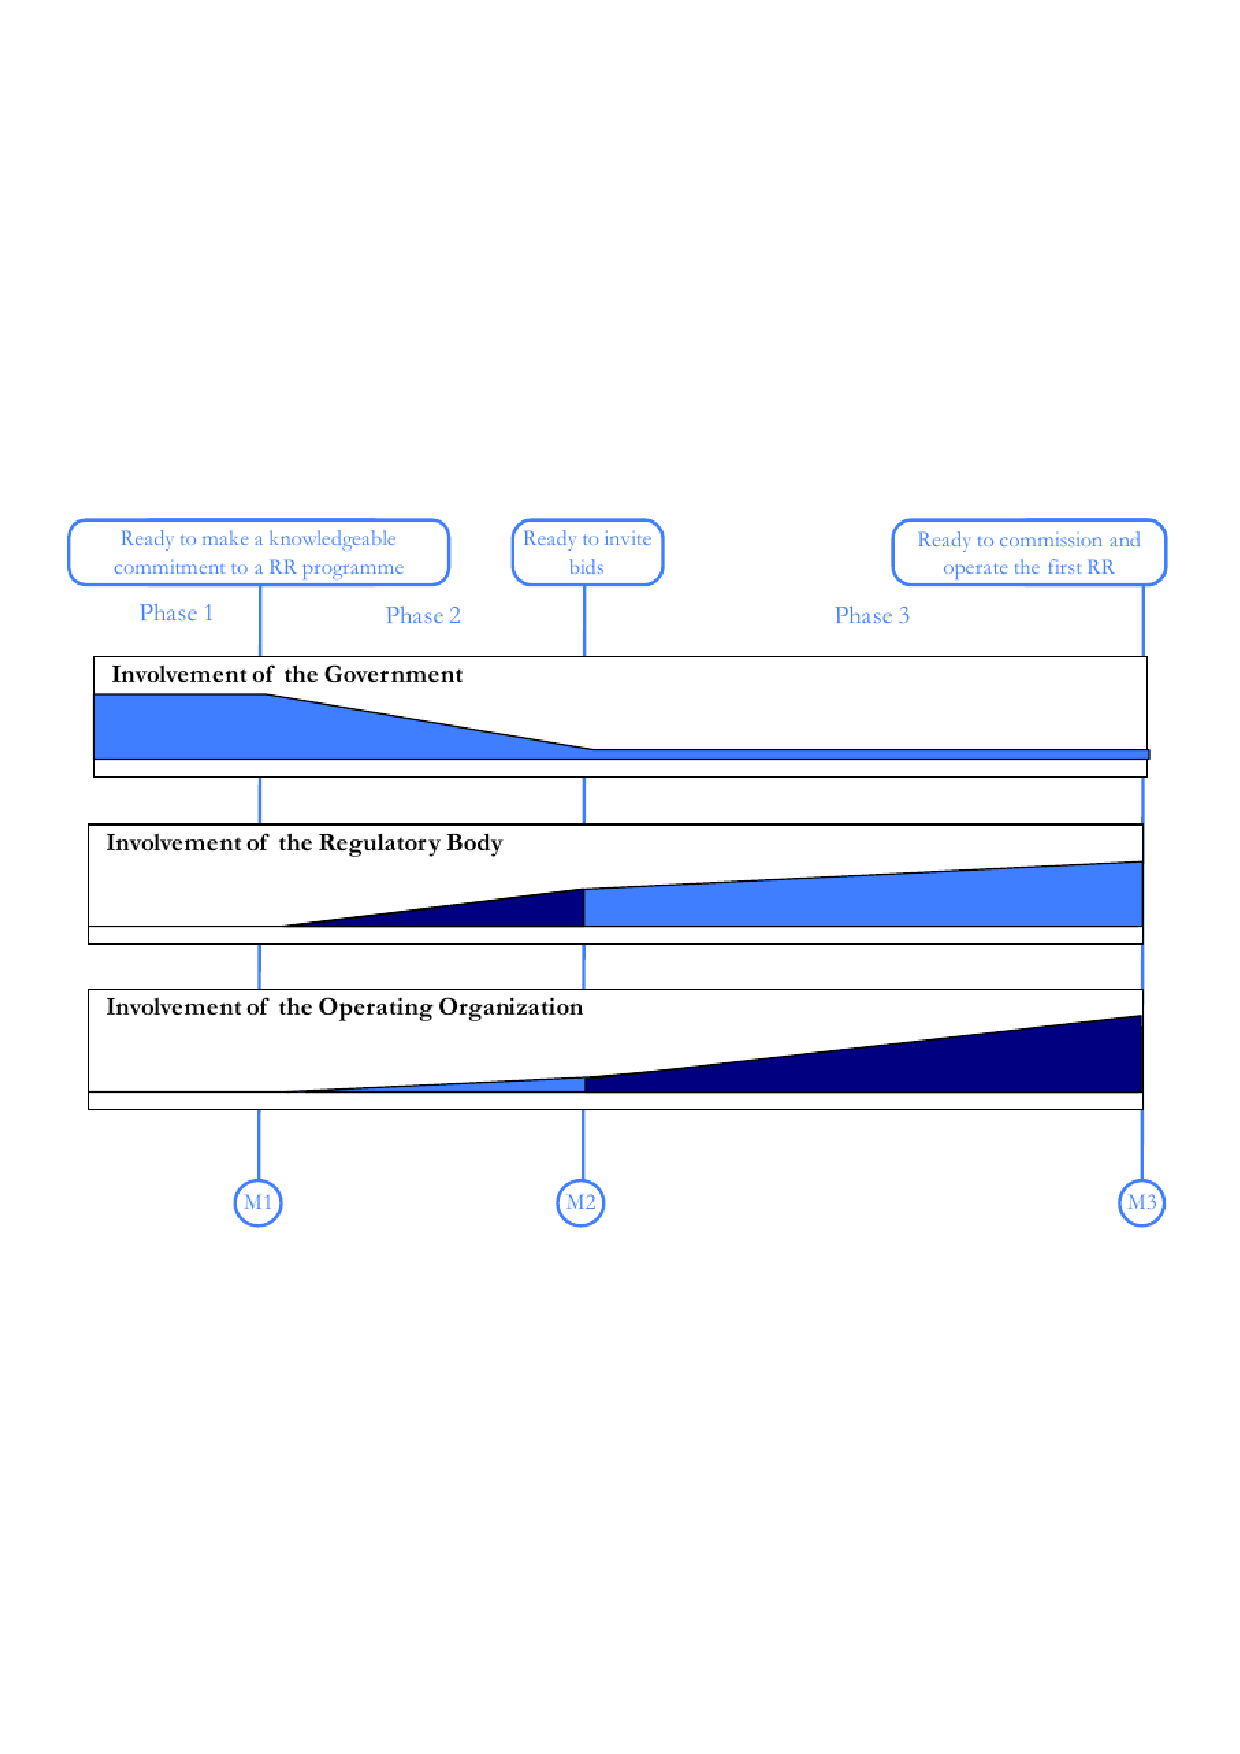
\includegraphics[width=0.7\linewidth,trim={1cm 8cm 1cm 8cm}, clip]{img/zapojeni_klicovych_hracu.pdf}
    \caption{Zapojení klíčových hráčů během života JZ.}
    \label{fig:2_15_zapojeni_klicovych_hracu}
\end{figure}

\textbf{Stát (vláda)}

\begin{itemize}
    \item Vydává zákony, buduje legislativní rámec, který upravuje provoz jaderných zařízení.
    \item Zavádí systém inspekcí a posuzování jaderných zařízení za účelem ověření dodržování platných předpisů a podmínek povolení.
    \item Vynucuje dodržování platných předpisů a podmínek povolení, včetně pozastavení, změny či zrušení povolení.
    \item Stát také zakládá státní regulační orgán (dozorčí orgán), který je zodpovědný za implementaci této politiky bezpečnosti a definici národních standardů.
    \item Vláda dále přijímá opatření pro nakládání RAO a vyřazování zařízení z provozu.
\end{itemize}

\textbf{Státní dozor}

\begin{itemize}
    \item Jmenovaný vládou státu.
    \item Je oprávněny k zajištění dohledu, včetně vydávání povolení, nad užíváním jaderné energie a ionizujícího záření, nakládání s radioaktivním odpadem a bezpečností dopravy.
    \item Provádí inspekce a hodnocení jaderných zařízení, aby se zajistilo dodržování platných předpisů a oprávnění.
    \item Prosazuje platné předpisy a povolení, včetně pozastavení, změny nebo zrušení povolení.
    \item Přezkoumává a posuzuje hodnocení bezpečnosti od provozovatele, a to jak před schválením, tak i periodicky během životnosti jaderného zařízení, a to i ve vztahu k úpravám, změnám ve využití a experimentálním činnostem důležitým pro bezpečnost.
    \item Nezávislost na držiteli licence a dalších organizacích.
    \item Plní informační roli pro veřejnost (laickou i odbornou).
\end{itemize}

\textbf{Provozovatel (držitel licence)}

\begin{itemize}
    \item Provozující organizace, která provádí jedno nebo více z umisťování, projektování, konstrukce, uvádění do provozu, provoz, úpravy a vyřazování jaderného zařízení z provozu = musí být schvalováno regulačním orgánem.
    \item Má zodpovědnost za bezpečnost zařízení.
    \item Provozující organizace by měla stanovit vlastní politiku v souladu s požadavky státu, které udělují otázkám bezpečnosti nejvyšší prioritu a podporují silnou kulturu jaderné bezpečnosti.
    \item Záměr vybudovat jaderné zařízení (feasibility study) je jediná etapa, která nevyžaduje autorizaci a nemusí projít licenčním řízením.
    \item Zajišťovat odpovídající výcvik a školení pracovníků.
    \item Vytvořit postupy a zajistit prostředky pro zajištění bezpečnosti zařízení za všech podmínek.
    \item Ověřit návrh zařízení a zajistit odpovídající kvalitu vybavení a činností souvisejících s provozem.
    \item Správa radioaktivních odpadů produkovaných při provozu.
\end{itemize}

\textbf{Zapojení klíčových hráčů}

Vláda a státní dozor mají zodpovědnost za ustanovení legislativního rámce pro ochranu obyvatelstva i životního prostředí před ohrožením plynoucím z provozu jaderných zařízení.

Držitel licence má přímou zodpovědnost za dodržování bezpečnosti a povinnost zajistit bezpečný provoz zařízení.

Mezi další významné hráče patří IAEA.

\subsubsection{International Atomic Energy Agency (IAEA)}

\begin{itemize}
    \item Cílem IAEA je spolupracovat s členskými státy a mezinárodními partnery na podpoře bezpečného, zabezpečeného a mírumilovného využívání jaderných technologií.
    \item IAEA podporuje a zároveň kontroluje využívání jaderné energie.
    \item ČR je člen od 1993.
\end{itemize}

\textbf{Role IAEA -- Záruková proces}

\begin{itemize}
    \item Smlouva o nešíření jaderných zbraní: The Treaty on the Non-Proliferation of Nuclear Weapons (NPT), 2005.
    \item Možnost kontrolovat plnění závazků Smlouvy o nešíření jaderných zbraní je mezi IAEA a jednotlivými státy upravena právními dohodami.
    \item NPT nejaderné státy:
    \item NPT jaderné státy: Čína, Francie, Rusko, UK a USA
    \item Non-NPT státy (státy, které nepodepsaly dohodu o nešíření jaderných zbraní): Indie, Izrael, Pákistán
\end{itemize}

\textbf{Role IAEA -- Bezpečnost a zabezpečení}

\begin{itemize}
    \item	Poradenství pro členské země, využití široké členské základy a rozsáhlé množství zkušeností s mírovým využitím jaderné energie.
    \item	Formuluje doporučení, vhodné praktiky.
    \item	Sdílení informací.
    \item	Pomoc jednotlivým státům na jejich žádost.
\end{itemize}

\textbf{Doporučení IAEA}

\begin{itemize}
    \item \textbf{Safety standards series} = Přímé podklady pro tvorbu národní legislativy nebo bezpečnostní dokumentace reaktoru, hierarchicky členěné do tří kategorií:
    \begin{itemize}
        \item \textbf{Safety fundamentals} = Základní bezpečnostní cíle a principy ochrany a bezpečnosti.
        \item \textbf{Safety requirements}:
        \begin{itemize}
            \item Rozvíjí základy specifikované v SF.
            \item Definují požadavky nezbytné pro zajištění bezpečnosti obyvatelstva a ŽP teď i v budoucnosti.
            \item Jejich formulace usnadňuje začlenění do národní legislativy.
        \end{itemize}
        \item \textbf{Safety guides}:
        \begin{itemize}
            \item Poskytují návod, jak splnit bezpečnostní požadavky.
            \item Představují mezinárodní doporučení a odrážejí nejlepší praktiky, které pomáhají dosáhnout vysokého stupně bezpečnosti.
        \end{itemize}
    \end{itemize}
    \item \textbf{Safety reports series}, Nuclear energy series, Technical reports series nebo Technical documents = Věnují se různým aspektům návrhu, výstavy a provozu jaderných zařízení, doplňují a rozpracovávají doporučení z dokumentů Safety standards series.
\end{itemize}

\subsubsection{SÚJB}

= Státní úřad pro jadernou bezpečnost. Nezávislý ústřední orgán státní správy a dozoru ČR. Garantuje adekvátní úroveň bezpečnosti technologií v ČR.

\begin{itemize}
    \item Úřad je podřízen vládě ČR a má samostatný rozpočet, který schvaluje Parlament ČR.
    \item V čele je předseda, který je jmenovaný vládou ČR (od 1.11.1999 Drábová).
    \item pravomoci a postavení srovnatelné s ministerstvy, v čele předseda (jmenuje a odvolává vláda), podléhá zákonu o státní službě, zastoupení ve vládě předsedou vlády, tj. je podřízen premiérovi.
    \item Nezávislý orgán státní správy.
    \item Normotvorná činnost, kontrola.
    \item Vykonává státní správu a dozor nad využíváním jaderné energie a IZ a v oblasti nešíření jaderných, chemických a biologických zbraní.
    \item Stanovuje základní podmínky zajištění JB, RO, HP a FO.
    \item Působnost útvaru upravuje At. zákon 263/2016 Sb. a částečně pak zákon o územním plánování a stavebnmím řádu nebo také trestní zákon či původní znění At. zákona v věci odpovědností za jaderné škody.
    \item Hlavní sídlo v Praze, lokální pracoviště -- ETE a EDU.
\end{itemize}

\textbf{Působnost SÚJB}

\begin{itemize}
    \item Povolování výkonu činností (umisťování a provoz jaderných zařízení a pracoviště s velmi významnými zdroji IZ, nakládání se zdroji IZ a RAO či přepravě JM a RN zdrojů).
    \item Schvalování dokumentace vztahující se k zajištění JB, RO, monitorování radiační situace, ZRMU, zabezpečení a nešíření jaderných zbraní, LaP, přeprava JM a vybraných RN zdrojů.
    \item Stanovení podmínek a požadavků RO obyvatel a pracovníků se zdroji IZ (stanovení limitů ozáření, vymezení KP), stanovení zóny HP a požadavků na RMU.
    \item Sledování stavu ozáření obyvatelstva a pracovníků se zdroji IZ.
    \item Vedení státního systému evidenc a kontroly JM, statních systému evidence držitelů povolení, dovážených a vyvážneých vybraných položek, zdrojů IZ,...
    \item Spolupráce s IAEA.
\end{itemize}

Tři sekce, které vycházejí z legislativou definovaných činností:

\begin{itemize}
    \item \textbf{Sekce jaderné bezpečnosti} = zabývá se především kontrolou jaderných zařízení, hodnocením jaderné bezpečnosti a nakládáním s vyhořelým jaderným palivem a radioaktivním odpadem.
    \item \textbf{Sekce radiační ochrany} = zahrnuje kontrolu zdrojů záření, radiační ochranu palivového cyklu a monitorování. 
    \item \textbf{Sekce řízení a technické podpory} = má na starost kontrolu nešíření zbraní hromadného ničení a dále zahrnuje odbory, které zajišťují provoz SÚJB, jako jsou ekonomický úsek a právní oddělení.
\end{itemize}

\subsection{Legislativní rámec}

\textit{Pozn.: Dobré asi vědět definici IZ, když se to všude objevuje v legislativě}

\textbf{Ionizující záření} = proud hmotných části nebo elektromagnetického záření doprovázející změnu energetického stavu nebo složení jádra atomu + může vyvolávat změny ve struktuře hmoty, a tedy i v buňkách živých tkání

Účinky IZ:

\begin{itemize}
	\item \textbf{Deterministické/prahové} (potřeba zabít dostatečné množství buněk) = smrt, nemoc z ozáření, popálení, lze regulovat udržením dávek pod prahem, s rostoucí dávkou roste účinek.
	\item \textbf{Stochastické} = buňka není zabita, ale pouze přeprogramována: leukémie, rakovina; nelze regulovat, pouze omezovat; s rostoucí dávkou roste pravděpodobnost vyskytnutí.
\end{itemize}

Cíl jaderného práva = chránit člověka a životní prostředí před škodlivými účinky IZ. Hlavní součásti infrastruktury jaderné bezpečnosti (analogie antického chrámu):

$\rightarrow$ Hlavní sloupy: kompetentní dozor, patřičná úroveň výzkumu a vývoje, inteligentní a schopný provozovatel.

$\rightarrow$ Základová deska: mezinárodní spolupráce a zpětné vazby z partnerských hodnocení, kultura bezpečnosti.

$\rightarrow$ Propojení prvních dvou sloupů skrze SÚJB.

\textbf{Právní řád ČR:}

\begin{itemize}
    \item Ústava $\rightarrow$ Ústavní zákony $\rightarrow$ Zákony $\rightarrow$ Vyhlášky $\rightarrow$ Nařízení vlády $\rightarrow$ Normy.
    \item V ČR jsou kromě našich zákonů také závazné mezinárodní úmluvy a smlouvy + evropská legislativa.
    \item Platí, že bezpečnost jaderných elektráren je v pravomoci jednotlivých států.
\end{itemize}

\subsubsection{Atomové právo}

= Soustava speciálních právních norem vytvořených pro regulaci chování právnických a fyzických osob zabývajících se činnostmi spojenými se štěpnými materiály, IZ a ozářením z přírodních zdrojů.

= Systém právních předpisů: regulace mírového využívání JE a IZ, At. zákon definuje základy a vymezuje, avšak dále jsou přiřazeny tzv. prováděcí právní předpisy (vyhlášky), které se specializují a podrobněji popisují konkrétní problematiku.

$\rightarrow$ mezinárodní a evropské kořeny

$\rightarrow$ implementace mezinárodní doporučení

\textbf{Klíčové oblasti}

\begin{itemize}
    \item Vydávání povolení k jednotlivým činnostem souvisejícím s využíváním jaderných technologií a stanovení požadavků pro zisk/udržení tohoto povolení.
    \item Stanovení povinností, které je nutno při těchto činnostech dodržovat.
    \item Výkon státní správy a dozoru.
    \item Nápravná opatření.
    \item Odpovědnost za jaderné škody.
    \item Ochrana proti přírodnímu ozáření.
    \item Uvádění/uvolňování radionuklidů do životního prostředí.
\end{itemize}

\subsubsection{České atomové právo}

V dnešní době je platný Zákon č. 263/2016 Sb., atomový zákon (účinnost od roku 2017) s tím, že se připravuje další nová verze 

Předchozí verzí je Zákon č. 19/1997 Sb., o mírovém využívání jaderné energie a IZ (atomový zákon) a o změně a doplnění některých zákonů (dnes platná a účinná jen jeho ustanovení o odpovědnosti za jadernou škodu).

Atomový zákon jako takový obsahuje dále prováděcí vyhlášky, jež jsou upřesňující vůči nějaké kategorii (vyhláška k RMU, vyhláška o umístění jaderného zařízení, vyhláška o evidenci a kontrole JM, vyhláška o požadavcích na projekt jaderného zařízení apod.)

\textbf{Atomový zákon}

Tři typy regulační nástrojů:

\begin{itemize}
	\item Povolení = individuální správní akt SÚJB.
	\item Registrace = evidenční/registrační úkon SÚJB.
	\item Ohlášení = informační úkon vůči SÚJB.
\end{itemize}

Zákonem je dále stanovena nutná odpovídající kvalifikace pracovníků při mírovém využívání jaderné energie a IZ: zvláštní odborná způsobilost, vybraní pracovníci, zkoušky (v legislativě je definován například operátor či provozní reaktorový fyzik).

členění dle typů aktivit při mírovém využívání jaderných technologií (využívání jaderné energie, činnosti v rámci expozičních situací, nakládání s RA odpadem, schvalování typu a přeprava, zvládání RMU, zabezpečení, nešíření jaderných zbraní, ...)

\textbf{Vydávání povolení pro celý životní cyklus JZ} 

Opět probíhá skrze Atomový zákon s využitím jeho 18 prováděcích vyhlášek, v jejichž souladu vydání povolení probíhá.

\begin{itemize}
	\item Jaderné zařízení:	
	$\rightarrow$ Stavba, jehož součástí je jaderný reaktor využívající řetězovou jadernou reakci
	$\rightarrow$ Sklad VJP, sklad čerstvého paliva, obohacovací závod, závod na výrobu jaderného paliva, sklad RA odpadu, úložiště RA odpadu
	$\rightarrow$ Největší jaderná zařízení v čR: Temelín, Dukovany, sklad čerstvého paliva v ETE, sklad VJP v EDU a ETE
	
	\item životní cyklus jaderného zařízení:	
	$\rightarrow$ Období vykonávání činnosti souvisejících s využíváním jaderné energie od umístění až po vyřazení (umístění, výstavba, fyzikální a energetické spouštění, zkušební provoz, provoz, jdnotlivé etapy vyřazování z provozu).

	\item Licenční a povolovací diagram:
	
	$\rightarrow$ Povolení k umístění, územní rozhodnutí, povolení k výstavbě, stavební povolení, první fyzikální spouštění, první energetické spouštění, zahájení zkušebního provozu, kolaudační souhlas, povolení k zahájení provozu JZ, provoz, jdnotlivé etapy vyřazování z provozu. 
    $\rightarrow$ Povolení je nutno vydávat/obdržet/žádat si o: při každém provedení změny ovlivňující jadernou bezpečnost, technickou bezpečnost a fyzickou ochranu jaderného zařízení.

	\item Projekt:	
	$\rightarrow$ Dokumentovaný návrh JZ a postupy a návody pro činnost související s využíváním jaderné energie během životního cyklu JZ.	
	$\rightarrow$ Po celou dobu životního cyklu musí být zajištěna jaderná bezpečnost, radiační ochrana, uplatnění ochrany do hloubky, odolnost a ochrana JZ, ...
    $\rightarrow$ Součástí je vždy provozní/prováděcí bezpečností zpráva PrBZ.
    
    \item Povinnosti držitele povolení:
    $\rightarrow$ Oznamovat úřádu neprodleně každou změnu nebo událost důležitou z hlediska JB, RO, technické bezpečnosti, monitorování radiační situace, ZRMU, zabezpečení a nakládání s JM.
    $\rightarrow$ Vyšetřit neprodleně každé porušení at. zákona a přijmout opatření k nápravě a zabránění opakování takové situace.
    $\rightarrow$ Hodnoti JB, RO, technickou bezpečnost, monitorování radiační situace, ZRMU a zabezpečení.
    $\rightarrow$ Zajistit výkon činností důležitých z hlediska JB a RO vybranými pracovníky.
    $\rightarrow$ Sledovat, měřit, hodnoti, ověřovat a zaznamenávat veličiny a skutečnosti důležité z hlediska bezpečnosti a informace o nich uchovávat a předávat úřadu.
    $\rightarrow$ Zajistit plnění bezpečnostních cílů a bezpečnostních funkcí a principů bezpečného využívání jaderné energie.
    $\rightarrow$ Poskytovat součinnost inspektorům IAEA a Evropské komise.
    $\rightarrow$ Pravidelně, systematicky a ověřitelným způsobem provádět hodnocení úrovně JB, RO, moitorování radiační situace, ZRMu a zabezpečení + přípdné zvláštní hodnocení, které je prováděno jen v případě před provedením změny při využívání jaderné energie.
    $\rightarrow$ Dále se sem vážou povinosti oznamovat když dojde k havárii, radiační nehodě, porušení LaP, RMU, čerpání LaP.
\end{itemize}



\subsubsection{Mezinárodní atomové právo}

Mezinárodní spolupráce: IAEA, NEA, WENRA (West European Nuclear Regulators Association), ICRP (International Commission on Radiological Protection), HERCA (Heads of the European Radiological Protection Competent Authorities), WANO (The World Association of Nuclear Operators).

Globální scéna jaderné bezpečnosti:

$\rightarrow$ Národní jaderný dozor zodpovídá za to, že provozovatel zaručuje bezpečnost jaderných zařízení.
$\rightarrow$ Požadavky mezinárodních smluv a úmluv, spojené programy výzkumu a vývoje.
$\rightarrow$ Mezinárodní standardy bezpečnosti.
$\rightarrow$ Účastníci globální scény: mezinárodní organizace (IAEA), asociace dozorů, asociace sdružující provozovatele (WANO), asociace výzkumu a vývoje, veřejnost (sociální sítě a média).

Mezinárodní doporučení:
$\rightarrow$ Jsou právně nezávazná, ale je moudré se jimi řídit (pak se ostatní mračí).

\textbf{Euroatom} = evropské společenství pro atomovou energii

6 zakládajících států (BE, NL, FR, LUX, DE, IT), dnes 27. 

Poslání Euratomu = přispět k vytvoření podmínek nezbytných pro rychlé vybudování a růst jaderného průmyslu, ke zvýšení životní úrovně v členských státech a k rozvoji vztahů s ostatními zeměmi.
